\subsection{LK 3D}\label{subsec:lk3d-results}
%%%%%%%%%%%%%%%%%%%%%%%%%%%%%%%%%%%%%%%%%%%%%%%%%%%%%%%%%%%%%%%%%%%%%%%%%%%%%%%%
%%%%%%%%%%%%%%%%%%%%%%%%%%%%%%%%%%%%%%%%%%%%%%%%%%%%%%%%%%%%%%%%%%%%%%%%%%%%%%%%
\begin{figure*}[t!]
        \centering
        \begin{subfigure}{0.3\textwidth}
                \centering
                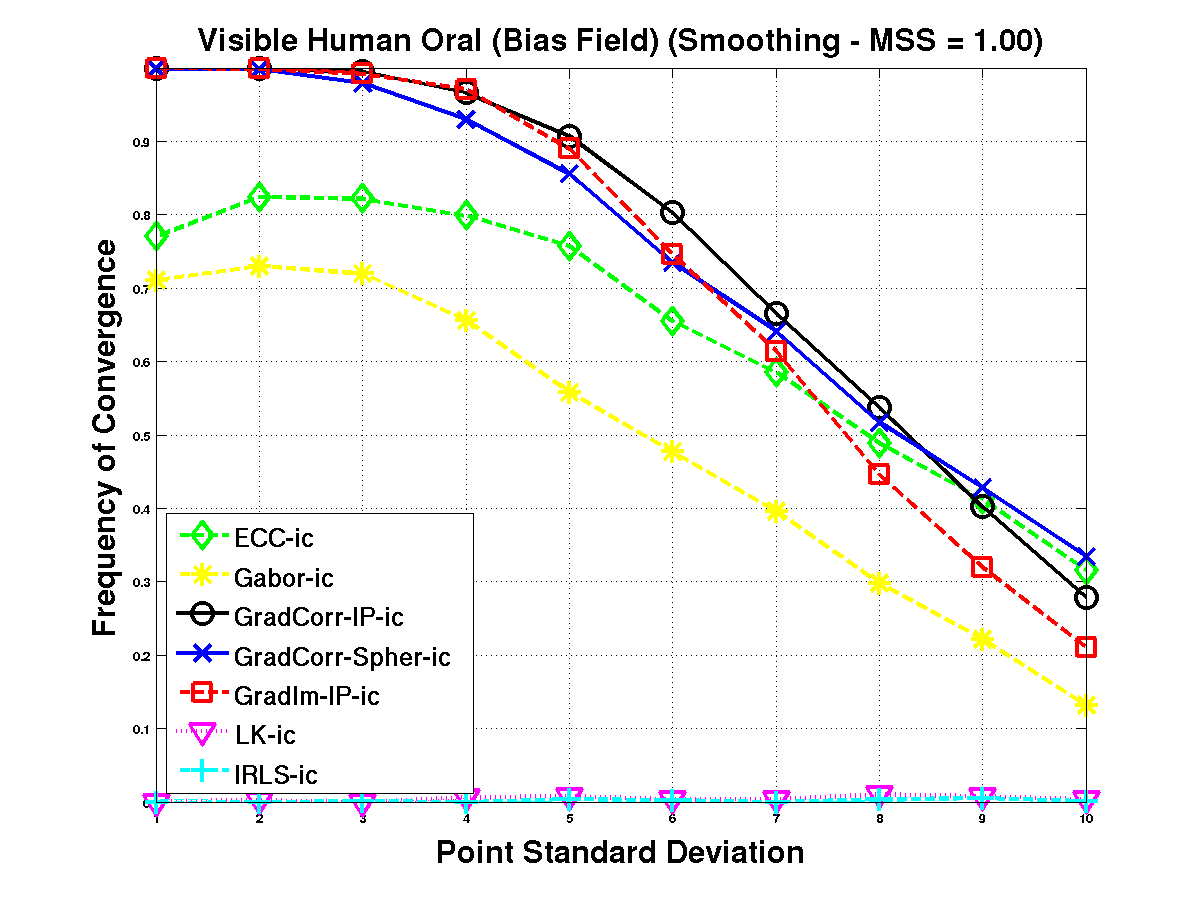
\includegraphics[width=\textwidth]{images/results/biasfield}
                \subcaption{}
                \label{fig:results-biasfield}
        \end{subfigure}
        \begin{subfigure}{0.3\textwidth}
                \centering
                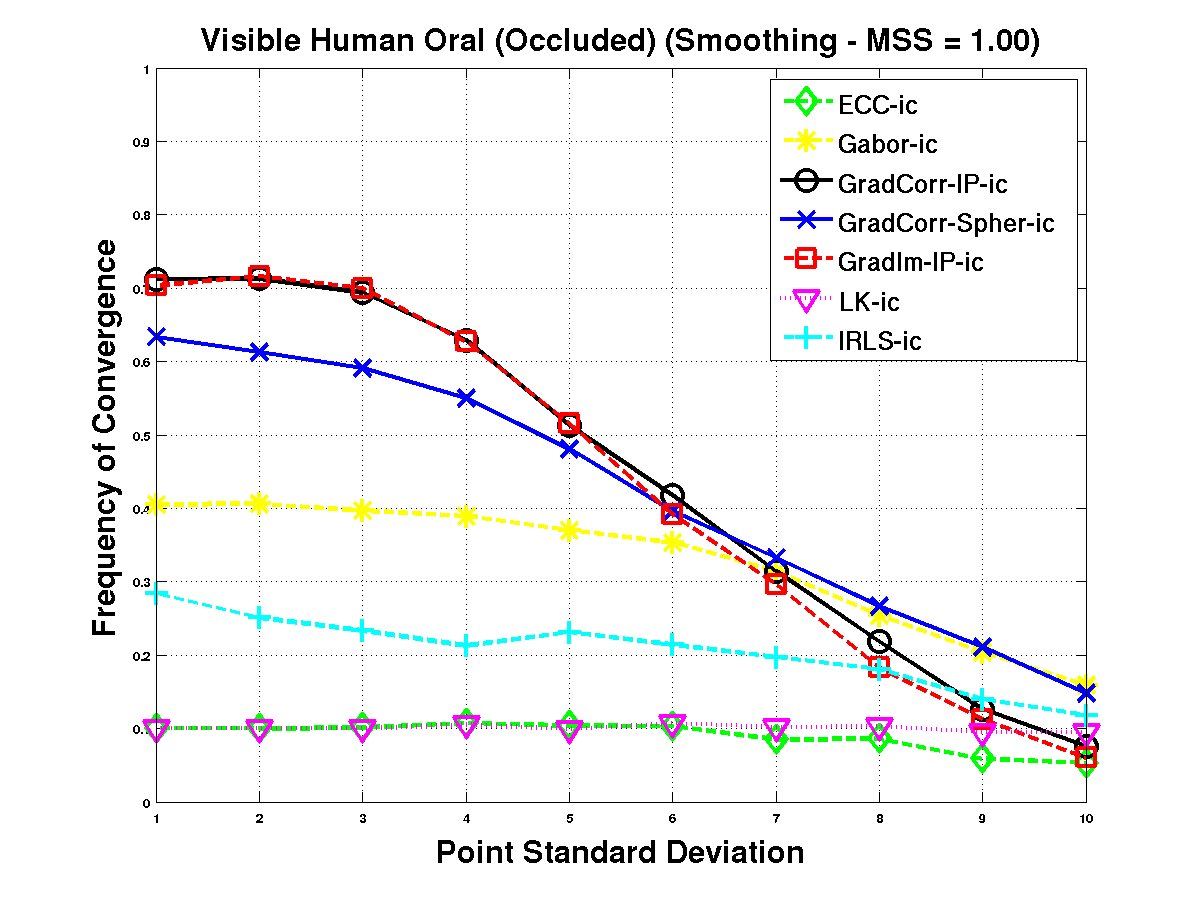
\includegraphics[width=\textwidth]{images/results/occlusion}
                \subcaption{}
                \label{fig:results-occlusion}
        \end{subfigure}
        \begin{subfigure}{0.3\textwidth}
                \centering
                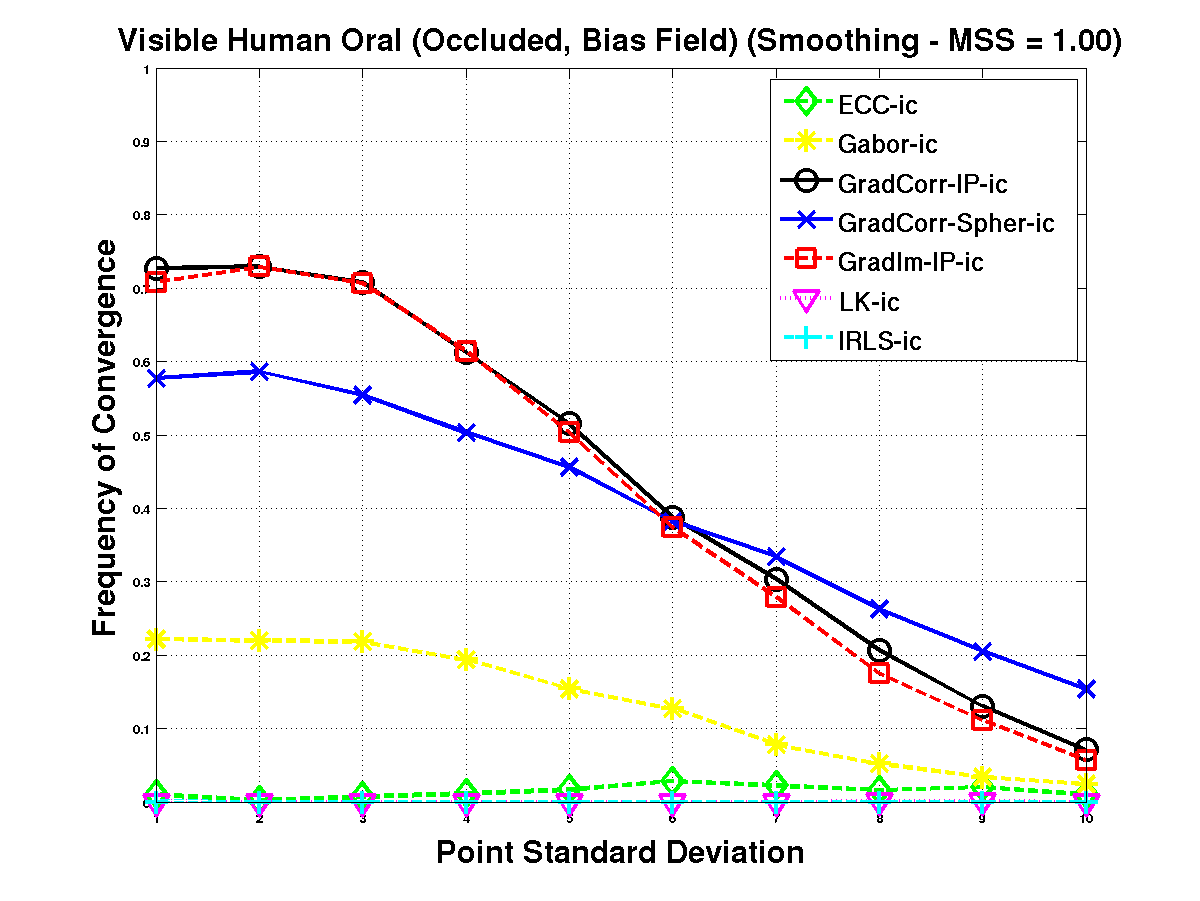
\includegraphics[width=\textwidth]{images/results/occlusion-biasfield}
                \subcaption{}
                \label{fig:results-occlusion-biasfield}
        \end{subfigure}
        \caption{Average frequency of convergence vs Point standard deviation for Visible Human data set. (a) Simulated bias field (b) Occlusions (c) Occlusions + bias field. ECC-ic: green-$\diamond$. Gabor-ic: yellow-*. GradCorr-IP-ic: black-o. GradCorr-Spher-ic: blue-x. GradIm-IP-ic: red-$\square$. LK-ic: magenta-$\bigtriangledown$. IRLS-ic: cyan-+}
        \label{fig:results-corrupted}
\end{figure*}
%%%%%%%%%%%%%%%%%%%%%%%%%%%%%%%%%%%%%%%%%%%%%%%%%%%%%%%%%%%%%%%%%%%%%%%%%%%%%%%%
We measure the performance of our algorithms within an extension of the evaluation framework proposed in \cite{RefWorks:10}. We used the Oral section from the Visible Human data set \cite{RefWorks:81} as the target area. We selected 10 different regions of interest and perturbed the points using Gaussian noise of standard deviation $\sigma$. Using the affine warp defined between the original and perturbed points, we generate a distorted image. Then, given a warp estimate, we compute the new template points and calculate the RMS error between the estimated and correct locations. The performance metric used to assess the algorithms is the average convergence rate for each fixed $\sigma = [1, 10]$, over each of the 10 regions of interest. An algorithm was considered to have converged if it had a final RMS point error of less than $n_1$ pixels after 30 iterations. For each template, 100 convergence tests were performed. Each image was smoothed using Gaussian smoothing before the calculation of derivatives.
%%%%%%%%%%%%%%%%%%%%%%%%%%%%%%%%%%%%%%%%%%%%%%%%%%%%%%%%%%%%%%%%%%%%%%%%%%%%%%%%
\begin{figure}[h]
    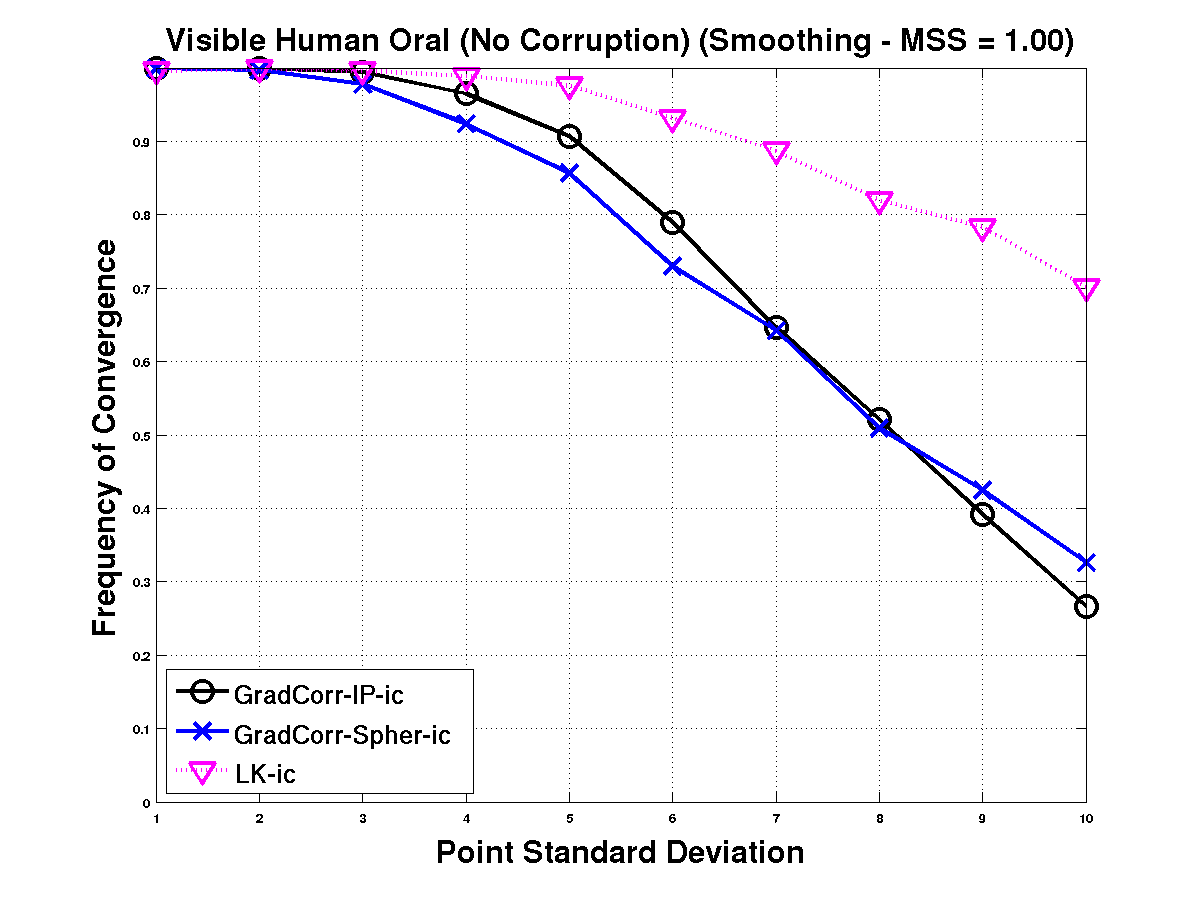
\includegraphics[width=0.45\textwidth]{images/results/nocorruption}
    \caption{Average frequency of convergence vs Point standard deviation for Visible Human data set with no corruption to the images. GradCorr-IP-ic: black-o. GradCorr-Spher-ic: blue-x. LK-ic: magenta-$\bigtriangledown$.}
    \label{fig:results-nocorruption}
\end{figure}
%%%%%%%%%%%%%%%%%%%%%%%%%%%%%%%%%%%%%%%%%%%%%%%%%%%%%%%%%%%%%%%%%%%%%%%%%%%%%%%%

%%%%%%%%%%%%%%%%%%%%%%%%%%%%%%%%%%%%%%%%%%%%%%%%%%%%%%%%%%%%%%%%%%%%%%%%%%%%%%%%
\subsection{Experiments Without Corruption}\label{subsec:results-nocorruption}
%%%%%%%%%%%%%%%%%%%%%%%%%%%%%%%%%%%%%%%%%%%%%%%%%%%%%%%%%%%%%%%%%%%%%%%%%%%%%%%%
In this subsection, we present our performance evaluation results obtained without applying any corruption to the 3D images. We considered alignments with errors of less than $n_1 = 1.0$ to have converged. We compared the performance of the inverse-compositional LK algorithm (LK-ic) with both forms of our algorithm, (GradCorr-IP-IC) and (GradCorr-Sph-IC). 

As Figure~\ref{fig:results-nocorruption} shows, the LK algorithm outperforms both of the proposed methods for this experiment. This result was in line with our expectations, as the distorted image is generated directly from the original image without any outliers. Since both of our proposed methods discard information in the form of the gradient magnitude, they inevitably perform worse than the LK algorithm. However, the difference between our two algorithms is negligible, which is expected given that they both discard the same amount of information.
%%%%%%%%%%%%%%%%%%%%%%%%%%%%%%%%%%%%%%%%%%%%%%%%%%%%%%%%%%%%%%%%%%%%%%%%%%%%%%%%
\subsection{Experiments With Corruption}\label{subsec:results-corrupted}
%%%%%%%%%%%%%%%%%%%%%%%%%%%%%%%%%%%%%%%%%%%%%%%%%%%%%%%%%%%%%%%%%%%%%%%%%%%%%%%%
In this subsection, we present three separate experiments: images with a simulated bias field, an occlusion and an occlusion + a simulated bias field. We include the performance of both of our algorithms (GradCorr-IP-IC) and (GradCorr-Sph-IC), as well as implementations of four other 2D alignment algorithms extended into 3D. The four algorithms we compared with are: the inverse-compositional LK algorithm (LK-ic) \cite{RefWorks:10}, the enhanced correlation coefficient algorithm (ECC-ic) \cite{RefWorks:59}, the iteratively re-weighted least squares algorithm (IRLS-ic) \cite{RefWorks:53} and the Gabor-Fourier LK algorithm (Gabor-ic) \cite{RefWorks:73}. We also include a variant of our algorithm that does not separate orientation and intensity. This algorithm, which we call (GradIm-IP-ic), uses the inner product relationship, but does not differentiate between intensities and gradients. This algorithm illustrates the performance improvement gained by solving a problem that accounts for the relationship between orientation and intensity.

Bias fields were simulated by multiplying an image region by a weighted filter that linearly interpolates between $1$ in the top-left of the image to $0.001$ in the bottom right. Each bias field was applied from left-to-right (x-y plane) across a slice (z-plane) in the 3D image, as shown in Figure~\ref{fig:biasfield-example}. Occluded sections were created synthetically by randomly placing image sections taken from the white matter area of the brain, and putting them into every slice of the 3D image, as shown in Figure~\ref{fig:occlusion-example}.
%%%%%%%%%%%%%%%%%%%%%%%%%%%%%%%%%%%%%%%%%%%%%%%%%%%%%%%%%%%%%%%%%%%%%%%%%%%%%%%%
\begin{figure}[b]
        \centering
        \begin{subfigure}{0.22\textwidth}
                \centering
                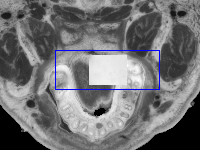
\includegraphics[width=\textwidth]{images/occluded-example}
                \subcaption{}
                \label{fig:occlusion-example}
        \end{subfigure}
        \begin{subfigure}{0.22\textwidth}
                \centering
                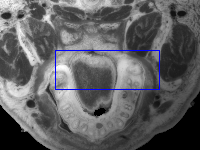
\includegraphics[width=\textwidth]{images/biasfield-example}
                \subcaption{}
                \label{fig:biasfield-example}
        \end{subfigure}
        \caption{(a) Example of an occluded slice of the 3D volume. (b) Example of a slice with a bias field applied to it. In both images the blue rectangle represents the template area being considered.}
        \label{fig:affine-examples}
\end{figure}
%%%%%%%%%%%%%%%%%%%%%%%%%%%%%%%%%%%%%%%%%%%%%%%%%%%%%%%%%%%%%%%%%%%%%%%%%%%%%%%%

Figure~\ref{fig:results-biasfield} shows that our proposed techniques outperform the state-of-the-art for bias field corruption. The non-robust methods of LK-ic and IRLS-ic are not able to cope with the intensity variation caused by the bias field. Gabor-ic copes reasonably well with this type of corruption due to the illumination invariant properties described in \cite{RefWorks:73}. ECC-ic also copes well, as the enhanced correlation coefficient performs a normalisation of the image pixels, which reduces the effect of the bias field. For larger values of $\sigma$, GradCorr-IP-IC outperforms GradIm-IP-IC by almost 10\%. This shows the benefit of considering both orientation as well as intensity for aligning images corrupted with a bias field.

Figure~\ref{fig:results-occlusion} shows that our proposed techniques are also very robust to occlusions. IRLS-ic performs better under these situations as it is able to discard some of the outliers that bias the alignment. The normalisation step in ECC-ic has no benefit in suppressing this sort of bias, and so it performs very similarly to the non-robust LK-ic algorithm.

Finally, in Figure~\ref{fig:results-occlusion-biasfield} we see that even under occlusion and illumination change, our proposed techniques perform impressively. Other than our techniques, only Gabor-ic is able to make any attempt at aligning the images, and even then only in 22\% of attempts. This is due to the illumination invariant properties of Gabor-ic described earlier.